\documentclass[]{article}
\usepackage{lmodern}
\usepackage{amssymb,amsmath}
\usepackage{ifxetex,ifluatex}
\usepackage{fixltx2e} % provides \textsubscript
\ifnum 0\ifxetex 1\fi\ifluatex 1\fi=0 % if pdftex
  \usepackage[T1]{fontenc}
  \usepackage[utf8]{inputenc}
\else % if luatex or xelatex
  \ifxetex
    \usepackage{mathspec}
  \else
    \usepackage{fontspec}
  \fi
  \defaultfontfeatures{Ligatures=TeX,Scale=MatchLowercase}
\fi
% use upquote if available, for straight quotes in verbatim environments
\IfFileExists{upquote.sty}{\usepackage{upquote}}{}
% use microtype if available
\IfFileExists{microtype.sty}{%
\usepackage{microtype}
\UseMicrotypeSet[protrusion]{basicmath} % disable protrusion for tt fonts
}{}
\usepackage[margin=1in]{geometry}
\usepackage{hyperref}
\hypersetup{unicode=true,
            pdftitle={Looking for evidence of a high burden of COVID-19 in the United States from influenza-like illness data},
            pdfauthor={Caitlin Rivers, Evan L. Ray, Graham C. Gibson, Estee Cramer, Nicholas G. Reich},
            pdfborder={0 0 0},
            breaklinks=true}
\urlstyle{same}  % don't use monospace font for urls
\usepackage{graphicx,grffile}
\makeatletter
\def\maxwidth{\ifdim\Gin@nat@width>\linewidth\linewidth\else\Gin@nat@width\fi}
\def\maxheight{\ifdim\Gin@nat@height>\textheight\textheight\else\Gin@nat@height\fi}
\makeatother
% Scale images if necessary, so that they will not overflow the page
% margins by default, and it is still possible to overwrite the defaults
% using explicit options in \includegraphics[width, height, ...]{}
\setkeys{Gin}{width=\maxwidth,height=\maxheight,keepaspectratio}
\IfFileExists{parskip.sty}{%
\usepackage{parskip}
}{% else
\setlength{\parindent}{0pt}
\setlength{\parskip}{6pt plus 2pt minus 1pt}
}
\setlength{\emergencystretch}{3em}  % prevent overfull lines
\providecommand{\tightlist}{%
  \setlength{\itemsep}{0pt}\setlength{\parskip}{0pt}}
\setcounter{secnumdepth}{0}
% Redefines (sub)paragraphs to behave more like sections
\ifx\paragraph\undefined\else
\let\oldparagraph\paragraph
\renewcommand{\paragraph}[1]{\oldparagraph{#1}\mbox{}}
\fi
\ifx\subparagraph\undefined\else
\let\oldsubparagraph\subparagraph
\renewcommand{\subparagraph}[1]{\oldsubparagraph{#1}\mbox{}}
\fi

%%% Use protect on footnotes to avoid problems with footnotes in titles
\let\rmarkdownfootnote\footnote%
\def\footnote{\protect\rmarkdownfootnote}

%%% Change title format to be more compact
\usepackage{titling}

% Create subtitle command for use in maketitle
\providecommand{\subtitle}[1]{
  \posttitle{
    \begin{center}\large#1\end{center}
    }
}

\setlength{\droptitle}{-2em}

  \title{Looking for evidence of a high burden of COVID-19 in the United States
from influenza-like illness data}
    \pretitle{\vspace{\droptitle}\centering\huge}
  \posttitle{\par}
    \author{Caitlin Rivers, Evan L. Ray, Graham C. Gibson, Estee Cramer, Nicholas G.
Reich}
    \preauthor{\centering\large\emph}
  \postauthor{\par}
      \predate{\centering\large\emph}
  \postdate{\par}
    \date{2020-03-06 21:42:44 CET}


\begin{document}
\maketitle

\hypertarget{introduction}{%
\subsection{Introduction}\label{introduction}}

In December 2019, an outbreak of a novel, SARS-like coronavirus was
detected in Wuhan, China. In the intervening weeks, case counts have
grown substantially. As of this writing, there are 95,333 confirmed
cases globally and at least 3,282 deaths of what is currently named
COVID-19 {[}1{]}. It is now understood that the virus transmits
efficiently from person to person, with R0 estimates above 2 and perhaps
as high as 3.7 {[}2, 3{]}.

Sustained human-to-human transmission has been observed outside of
China, and the possibility of unrecognized spread in the United States
and other countries cannot be ruled out at this stage. Emerging
phylogenetic data suggest that sequenced cases to date in the United
States and globally share a common ancestor between mid-November and
mid-December 2019. The same analyses suggest that some transmission
chains may have been progressing, undetected, in the Pacific northwest
of the United States since mid-January.{[}4{]} As an early effort to
explore the scenario of undetected spread in the United States, we
analyze publicly available data on influenza-like illness in the US.
Specifically, we compare the proportion of weighted influenza like
illness (wILI) that tests negative for influenza during the 2019-2020
flu season to trends from previous seasons. If it were the case that
COVID-19 were circulating unobserved in the United States, we might
expect to see in recent weeks a higher fraction of ILI specimens that
test negative for influenza compared to the same time in past seasons.

\hypertarget{methods}{%
\subsection{Methods}\label{methods}}

\hypertarget{data}{%
\paragraph{Data}\label{data}}

We downloaded publicly available ILINet and WHO-NREVSS data for US
Health and Human Services (HHS) regions (Figure 1) and states.

\begin{figure}
\centering
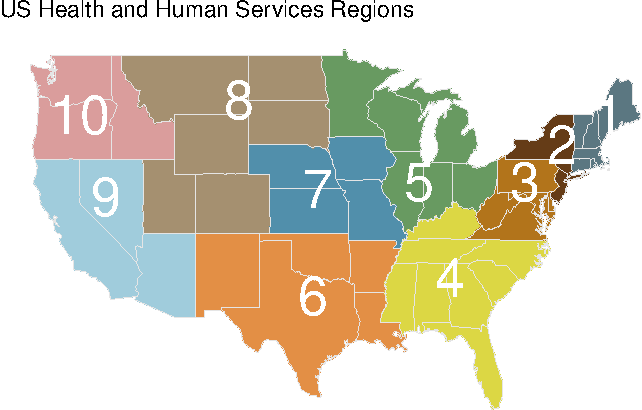
\includegraphics{ili-labtest-report_files/figure-latex/hhs-regions-map-1.pdf}
\caption{\label{fig:hhs-regions-map}US HHS Regions are made up of groups
of states.}
\end{figure}

From the ILINet dataset, we downloaded weighted influenza-like illness
(wILI), which measures the percentage of doctor's office visits at
sentinel providers that had the primary complaint of fever plus an
additional influenza-like symptom (cough, sore throat, etc\ldots{}). For
the WHO-NREVSS data, we obtained the total number of specimens tested by
participating clinical laboratories, as well as the percent of those
specimens that tested positive for influenza. We used 23 seasons of data
for HHS regions, beginning with the 1997/1998 season, and 10 seasons of
data for states, beginning with the 2010/2011 season. All data sources
are available at the weekly time-scale, defined as using the MMWR week
standard used by the CDC.

The code used to produce this report is available on GitHub at
\url{https://github.com/reichlab/ncov}.

\hypertarget{influenza-like-illness-not-attributable-to-influenza}{%
\paragraph{Influenza-like illness not attributable to
influenza}\label{influenza-like-illness-not-attributable-to-influenza}}

One possible measure of influenza illness not attributable to influenza
(ILI-) can be calculated as follows:

\[\text{ILI-} = (1 - \text{proportion of tests positive for influenza}) \times \text{wILI}\]

It is important to note that reported wILI can vary substantially due to
differences in the types of health care providers reporting into ILINet.
Therefore, some increases in reported wILI from one season to another
may be driven in part by changes in provider type make up. An
approximate way to adjust for this is by dividing reported wILI by the
baseline for a given region and season. Baselines for HHS regions are
provided by the CDC. Baselines for states are calculated as the average
of the first two weekly ILI observations for a given season, thinking
that this adjusts for any systematic adjustments to the provider mix in
each season. These baselines enable the following calculation of a
\textbf{r}elative ILI-.

\[\text{rILI-} = (1 - \text{proportion of tests positive for influenza}) \times \frac{\text{wILI}}{\text{baseline level for ILI}}\]

\hypertarget{measuring-anomalies-in-ili--during-a-season}{%
\paragraph{Measuring anomalies in ILI- during a
season}\label{measuring-anomalies-in-ili--during-a-season}}

We developed a metric to measure the degree to which a given ILI-
observation is significantly higher or lower than expectation, based on
past trends at similar times of the year. For each region and
season-week, we averaged observations from the past seasons (22 seasons
for regions, 9 for states) for the given season week and one season week
on either side and calculated the standard deviation based on these same
observations. We then computed ``z-scores'' as the number of standard
deviations above or below the average a particular rILI- observation is:
\[\text{Z} =  \frac{\text{rILI-} - \overline{\text{rILI-}}}{sd{\text{rILI-}}}\]

\hypertarget{results-discussion}{%
\subsection{Results \& Discussion}\label{results-discussion}}

This report uses data downloaded on March 06, 2020, with data reported
through February 29, 2020.

\hypertarget{regional-level-analyses}{%
\subsubsection{Regional-level analyses}\label{regional-level-analyses}}

We plotted ILI- and rILI- as a function of the week within each flu
season and stratified by region (Figure 2). Additionally, we plotted the
2019/2020 Z-scores for all regions as a function of week of season
(Figure 3).

In the last weeks of 2019 and first weeks of 2020, the observations of
ILI burden due to non-influenza pathogens (rILI-) have been, relative to
what has been observed in the past 22 seasons, above the seasonal
average. However, the measures of rILI- also have not been consistently
more than 3 standard deviations above the average (Figure 3).

These results do not particularly rule out any possibilities of COVID-19
transmission occuring in the US at the time of the most recent data
reporting or not. If COVID-19 were circulating widely in the US, these
data would seem to suggest that its incidence would be currently
relatively small, as it would not be adding much relative to levels of
rILI- observed in past seasons. However, it is hard to determine this
conclusively, as we have not performed an exhaustive analysis about what
other pathogens were or were not ciruclating in those past seasons.

If COVID-19 were to cause significant influenza-like illness in
subsequent weeks, we might expect the rILI- metric to increase and be
larger than previous seasons. However, media attention could also drive
more individuals with mild influenza-like illness symptoms to seek care
than usual even in the absence of widespread COVID-19 transmission in
the US. If these additional individuals seeking care were more likely to
have an illness not caused by influenza, then this could also drive up
the rILI- metric.

\begin{figure}
\centering
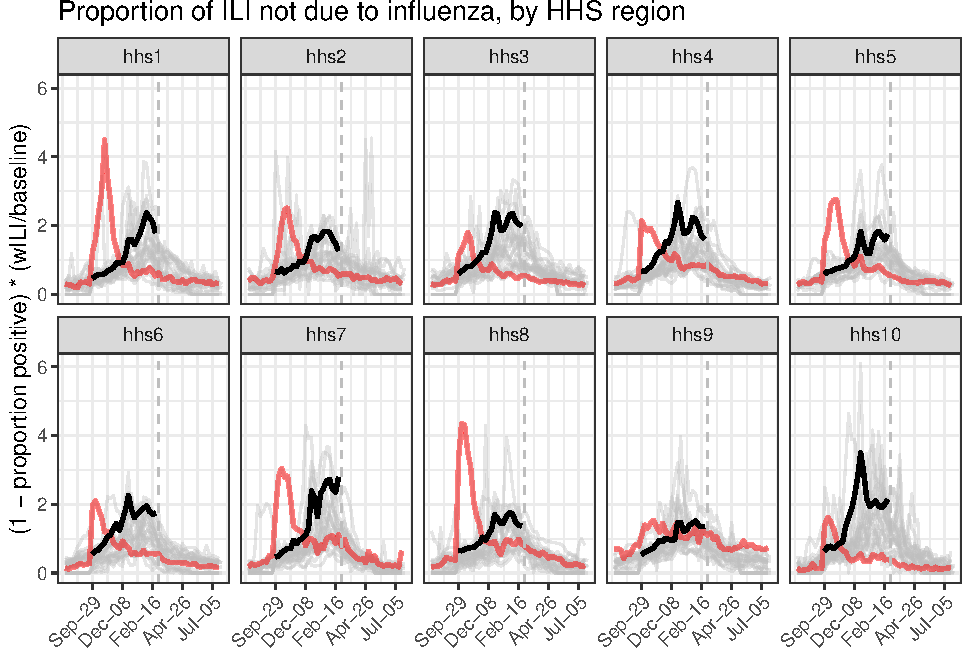
\includegraphics{ili-labtest-report_files/figure-latex/all-region-plot-ILI-1.pdf}
\caption{\label{fig:all-region-plot}US HHS Regions plots showing rILI-
values since the 1997/1998 season (grey lines) and the 2019/2020 season
(dark black line). The line highlighted in red is the 2009/2010 H1N1
pandemic season. The dates on the x-axis correspond to the dates for the
2019/2020 season, with previous seasons lined up approximately the same
time by week. The vertical dashed line shows the date at which this plot
was generated. The small gap between the current season's data and the
line indicates the lag in ILI reporting, typically one week.}
\end{figure}

\begin{figure}
\centering
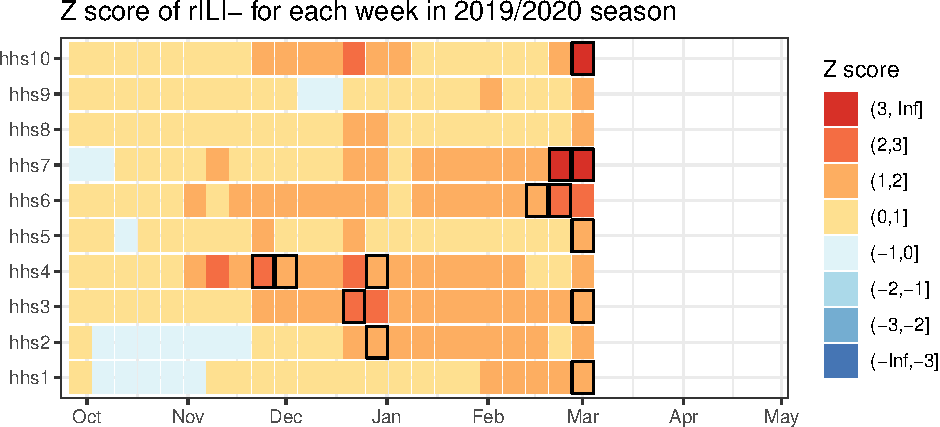
\includegraphics{ili-labtest-report_files/figure-latex/std-dev-analysis-1.pdf}
\caption{Figure showing Z scores by week for each HHS region. Tiles with
a dark black outline indicate locations where the observed rILI- was
higher in that week of the season than had ever been observed in the
last 22 seasons.}
\end{figure}

\hypertarget{state-level-analyses}{%
\subsubsection{State-level analyses}\label{state-level-analyses}}

The z-score calculations show a few states with systematically higher
than average observations (Figure 4). We think many of these may be
spurious, due to other systematic differences in reporting for this
season. Although at this time we do not have specific data to support or
refute this hypothesis.

We specifically compare two states with levels of community transmission
in the US, California and Washington (Figure 5). In California, levels
of ILI not due to influenza (rILI-) have been increasing in recent weeks
and were higher than they have ever been in February, although on par
with peaks in other seasons. In Washington, no anomalous levels of rILI-
have been detected in 2020.

\begin{figure}
\centering
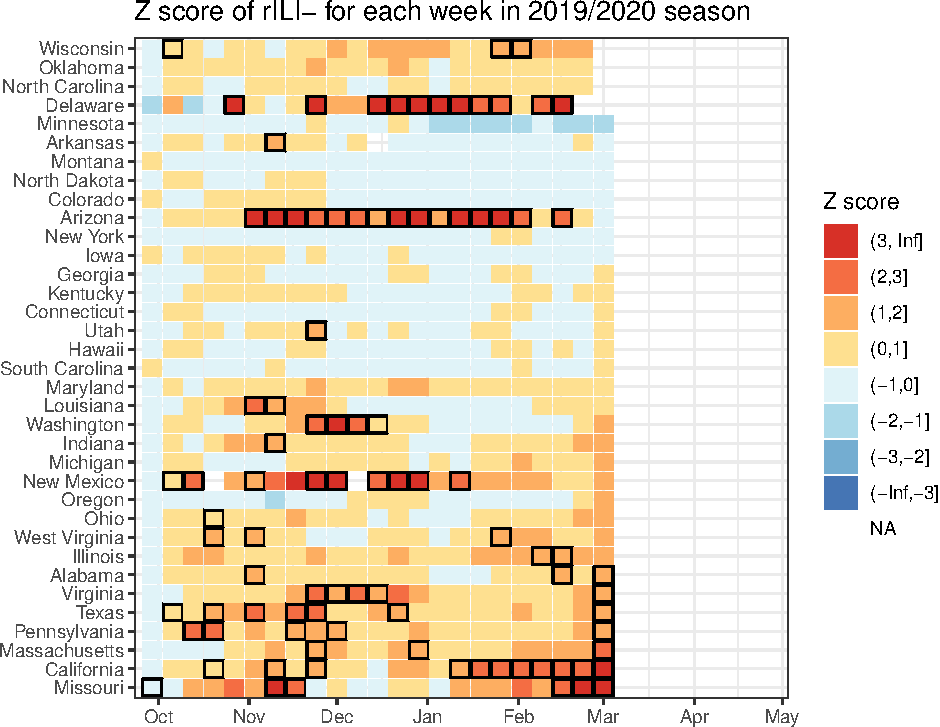
\includegraphics{ili-labtest-report_files/figure-latex/calc-avg-sd-all-states-1.pdf}
\caption{Figure showing Z scores by week for each state in the US that
has collected and tested more than 5000 specimens for influenza during
the 2019/2020 season. Tiles with a dark black outline indicate locations
where the observed rILI- was higher in that week of the season than had
ever been observed in the last 22 seasons. Some states have no reported
tests for a given week and so the rILI- is missing for that week. States
are sorted by z-score in the most recent week, with highest scores at
the bottom (states with missing z-scores for the most recent week are at
the top).}
\end{figure}

\begin{figure}
\centering
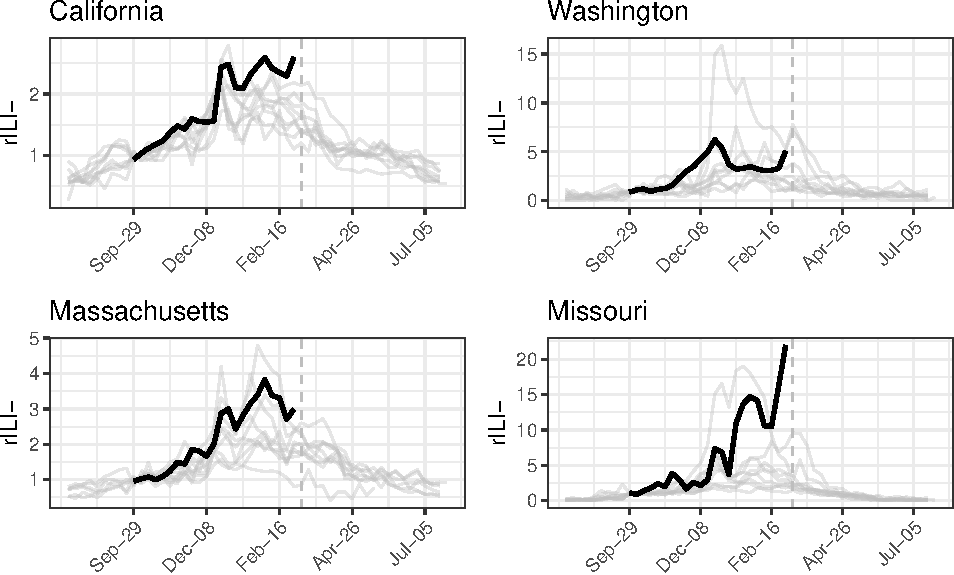
\includegraphics{ili-labtest-report_files/figure-latex/get-sd-data-1.pdf}
\caption{Selected individual state-level plots showing the proportion of
ILI not due to influenza over the current 2019/2020 season (dark black
line) and past 9 seasons, starting with 2010/2011.}
\end{figure}

\hypertarget{works-cited}{%
\subsection{Works Cited}\label{works-cited}}

{[}1{]}
\url{https://www.who.int/emergencies/diseases/novel-coronavirus-2019/situation-reports/}

{[}2{]} Yang, Y., Lu, Q., Liu, M., Wang, Y., Zhang, A., Jalali, N.,
Dean, N., Longini, I., Halloran, M. E., Xu, B., Zhang, X., Wang, L.,
Liu, W., \& Fang, L. (2020). Epidemiological and clinical features of
the 2019 novel coronavirus outbreak in China. MedRxiv,
2020.02.10.20021675. \url{https://doi.org/10.1101/2020.02.10.20021675}

{[}3{]} Imai, N., Cori, A., Dorigatti, I., Baguelin, M., Donnelly, C.
A., \& Riley, S. (n.d.). Report 3: Transmissibility of 2019-nCoV.
\url{https://www.imperial.ac.uk/media/imperial-college/medicine/sph/ide/gida-fellowships/Imperial-2019-nCoV-transmissibility.pdf}.

{[}4{]} Bedford T, Neher R, Hadfield J, Hodcroft E, Ilcisin M, M"uller
N. Genomic analysis of COVID-19 spread. Situation report 2020-03-04.
\url{https://nextstrain.org/narratives/ncov/sit-rep/2020-03-04}

\clearpage

\hypertarget{changelog}{%
\subsection{Changelog}\label{changelog}}

6 March 2020: updated for new ILI data, genomic commentary, some state
figures.

2 March 2020: Added state-level analysis, HHS region map, z-score code
and figure.

29 February 2020: updated for new ILI data. Minor rephrasing in intro.

21 February 2020: updated for new ILI data.

16 February 2020: updated to revise name of COVID-19, updated case
counts and ILINet data, added citations and revised statements about R0.

2 February 2020: Updated to include new ILINet data released on Friday,
Jan 31.

26 January 2020: Although our overall assessment has not changed and our
analysis has not been updated, we have updated the discussion to better
convey the level of uncertainty in our analysis. We also added a heavier
line for the 2019/2020 season in the figures.

25 January 2020: First version of report released.


\end{document}
